\documentclass[11pt,a4paper]{article}
\usepackage[utf8]{inputenc}
\usepackage[english]{babel}

\usepackage{graphicx}
\usepackage[english]{babel}
\usepackage[margin=0.85in]{geometry}
\usepackage{amsmath}
\usepackage{natbib}
\usepackage{hyperref}
\bibliographystyle{plainnat}
\usepackage{setspace}


% These are the configurable settings
% Please change them to make it fit your course
\def \institute {Institute / project name}
\def \authors { Youri Hoogstrate, \institute }

\def \servers {
\begin{itemize}
	\item \url{https://usegalaxy.org/}
	\item \url{https://bioinf-galaxian.erasmusmc.nl/galaxy/}
\end{itemize}
}
\def \datalibrarydirintroduction {
	TraIT Galaxy Training Materials
		$\rightarrow$
	TraIT Galaxy Training - 1: Introduction to Galaxy
}

\def \datalibrarydirrnaseqtuxedo {
	TraIT Galaxy Training Materials
		$\rightarrow$
	TraIT Galaxy Training - 3: RNASeq Tuxedo Pipeline
}

\def \datalibrarydirrnaseqadvanced {
	TraIT Galaxy Training Materials
		$\rightarrow$
	TraIT Galaxy Training - 5: Advanced RNA-Seq Analysis
}
% Configurations should be changed in this file

\begin{document}
\title{ \textit{\institute}\text{ }Galaxy Training: RNA-Seq DGE analysis \\
{ \large This practical aims to familiarize you with the Galaxy RNA-Seq analysis, the FastQ format and data collections (pairs).}}

\author{ \authors }
\maketitle

%\newpage
%\tableofcontents
%\newpage

%\doublespacing

\section*{Introduction}
Due to the rapid development of Galaxy, screenshots and results may be out of date. If you experience something like this, please report it as a bug at \url{https://github.com/ErasmusMC-Bioinformatics/galaxy-courses/issues}.


% It should describe:
% - server address(es)
% - whether to use specific training accounts or register one
% - a notice until when the server will be available or whether it will be accessible after the course
% - funding related notices
\section*{Preparations}
\subsection*{Open Galaxy}
Please open a web browser and navigate to your assigned Galaxy server:

\servers

\subsection*{Register for an account}
In the top menu bar, go to User and then choose Register (fig. \ref{fig:registration}). After registration, click on Analyze data in the top menu to return to the main screen.

\begin{figure}
 \center
  
\includegraphics[scale=0.6]{../figures/register_icon_1}
  \caption{\small{ The icons used in Galaxy to go to the registration page }}
  \label{fig:registration}
\end{figure}% Preparations should describe how to access which server

% Module QC/QA:
\section{RNA-Seq: QC/QA}
The very first step of an RNA-Seq analysis is the quality control and quality assurance. The sequencing data is usually provided in FASTQ format, which reports the sequenced bases and also describes per base the quality reflecting the probability it was measured correctly. However, different encodings are being used. Galaxy contains tools that assist you in determining and dealing with these formats by converting them to \textit{fastqsanger}.

\subsection{Paired end data as `pairs' within galaxy}
\textbf{Note: using `pairs' for storing paired end reads in galaxy is experimental but will become the common way doing analysis on paired end data.} \\
This section will only show how to do this.

For this module, create a new history and load the Shared Data (\textit{\datalibrarydirrnaseqadvanced}) files ``ctrl\_small\_1.fq'' and ``ctrl\_small\_2.fq'' and ``treat\_small\_1.fq'' and ``treat\_small\_2.fq'' into your history. As you may expect from the file names already, \verb|_1| and \verb|_2| indicate that these files are paired end and belong together:\\
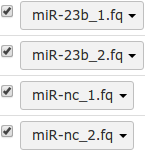
\includegraphics[scale=0.65]{figures/qc_01.png}\\
Hence, each pair of files belong to each other and we can treat them as pairs in galaxy. First you have to select the checkbox on top of the history ``\textit{Operations on multiple datasets}'', select the history items that belong to the pair of interest and then press the button \textit{For all selected...} to apply actions on multiple history items at once, select \textit{Build Dataset Pair}. Galaxy does not really know which one is the forward and which one is the reverse. Therefore make sure that \textbf{\_1 is forward} and \textbf{\_2 is reverse}. If galaxy does not choose the files correctly by it itself, use \text{Swap}. One of the samples has been treated with miR-23b and the other is a control. Make sure you use names that make this clear. After you have done this, you will see that you end up with 6 datasets in total, of which 2 pairs. To avoid confusion it is easier to hide the individual history items, leaving two items in the history:\\
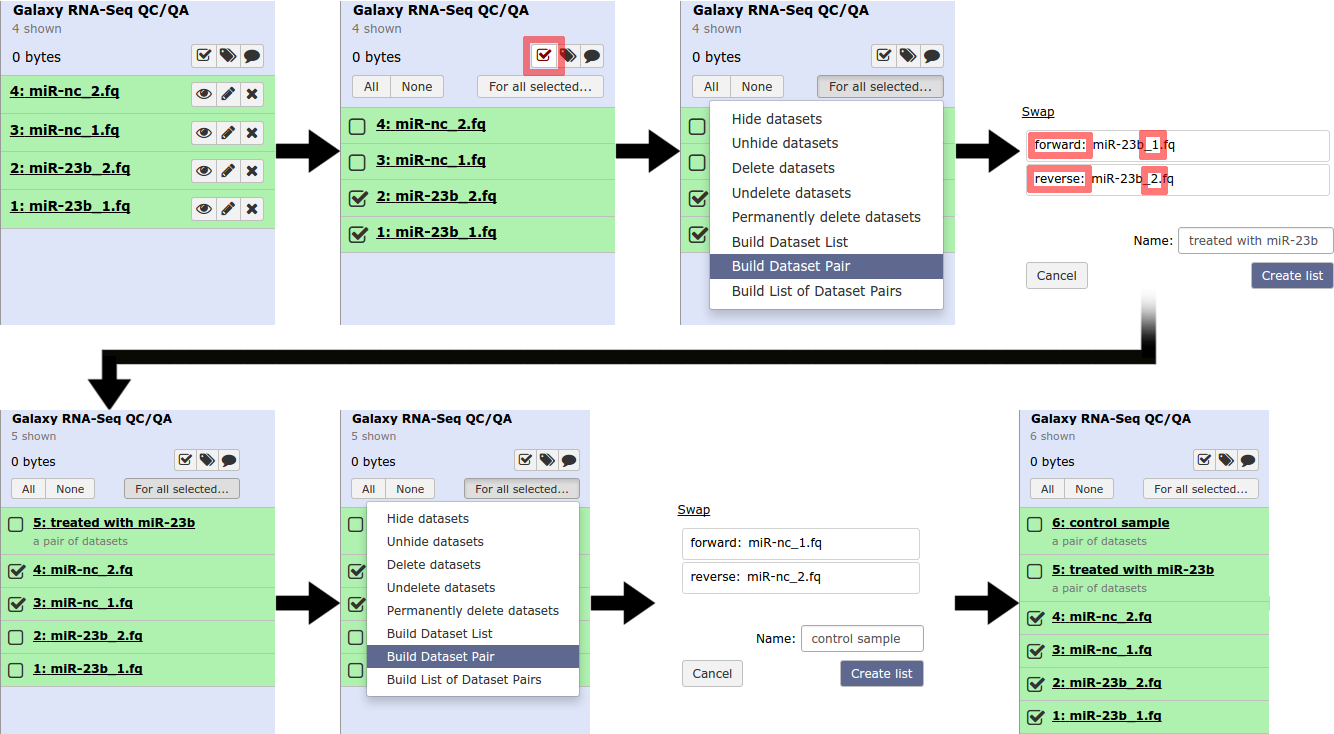
\includegraphics[width=\textwidth]{figures/qc_02.png}\\
\subsection{Fastq, Fastqsanger and FastQC}
To obtain statistics on the data, find the tool ``\textit{\underline{FastQC} Read Quality reports}''. This tool, originally developed for DNA-Seq analysis, makes several summaries of the data and reports the summary in a HTML page. By default FastQC selects the individual fastq files for analysis. This is because FastQC does analysis just on one fastq file. When we choose to select one of our pairs, galaxy will run FastQC twice and merge the results into a new pair. You can choose whether you want to run them as pair or as single file seperately, but make sure you run all of them to get an impression of the data. In the following figure it is demonstrated how to use FastQC in combination with pairs:\\
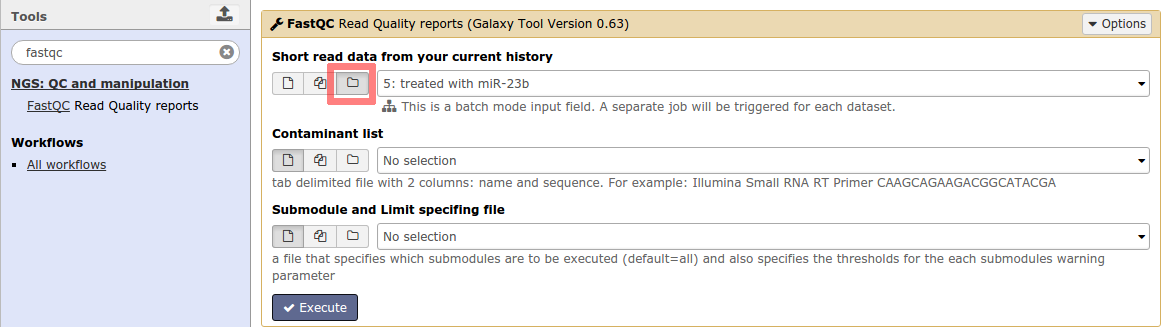
\includegraphics[width=\textwidth]{figures/qc_03.png}\\
What follows is a quality report (raw data and HTML report) for each FASTQ file. Open the miR23b (forward) FastQC report that contains \textit{\ldots: Webpage \ldots} in its name which should look similar to this:\\
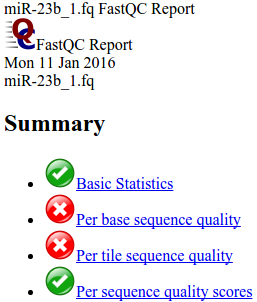
\includegraphics[scale=0.65]{figures/qc_04.png}\\
The galaxy history items are in the \textbf{fastq} format. This format is a general format that covers four specific subformats that differ in their quality encoding. Before we proceed with the next step it is important to understand the FASTQ encoding formats. They are described at the following website in section \textit{Encoding}:\\
\url{http://en.wikipedia.org/wiki/FASTQ\_format#Encoding}\\
In the FastQC report, scroll down to \textbf{Basic Statistics} and figure out what the \text{Encoding} is. This information is important because other tools want the specific subdatatype instead of `\textit{fastq}', so write the format as reported by FastQC down:\\
\verb|.......................................................|\\
The more or less standard encoding is \textit{fastqsanger}, which is the same encoding as \textit{Illumina 1.8} and \textit{Illumina 1.9}, also referred to as \textit{Illumina 1.8+}. To convert a fastq file into \textit{fastqsanger}, we use the tool ``\textit{\underline{FASTQ Groomer} converts between various FASTQ quality formats}''. In here, make sure the quality encoding you wrote down matches the one in the input field. Further, make sure you run it for each sample:\\
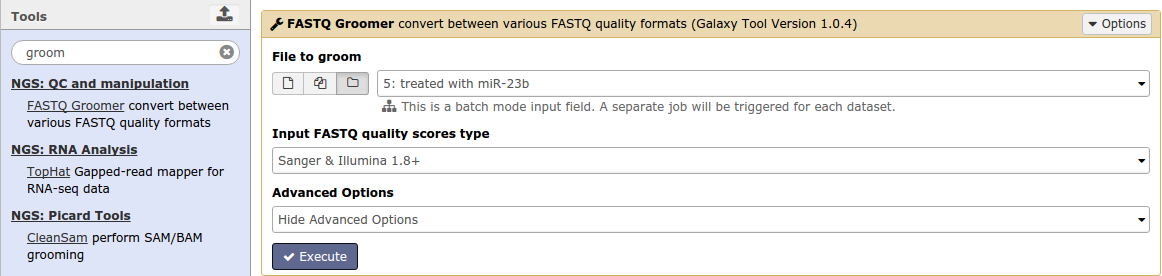
\includegraphics[width=\textwidth]{figures/qc_05.png}\\
This will add the groomed fastqsanger files to your history, with names that are not convenient. Please rename such that you can keep track of the sample name (miR23b/control) and, if you did not use pairs, whether the reads are forward or reverse.

If we go back to the FastQC webpage report, and look in section \textit{Per base sequence quality}, we see the average quality per base for all reads. The colors green, orange and red indicate whether the quality is considered good, okay, or bad. As you can see, the quality drops as the sequences get longer. It is important to realize that low quality bases will complicate alignment as well as SNP detection, because there will be more mismatches. To improve overall the base quality of the data, we would like to:
\begin{itemize}
	\item Trim the low quality bases from the ends
	\item Remove reads of which the average quality is too low
	\item Remove reads that are too short
\end{itemize}
A tool that covers all of this is ``\textit{\underline{Sickle} windowed adaptive trimming of FASTQ data}''. Because we have paired end data, we have to run it twice, once for miR-23b and once for the control. Run it with the following settings:\\
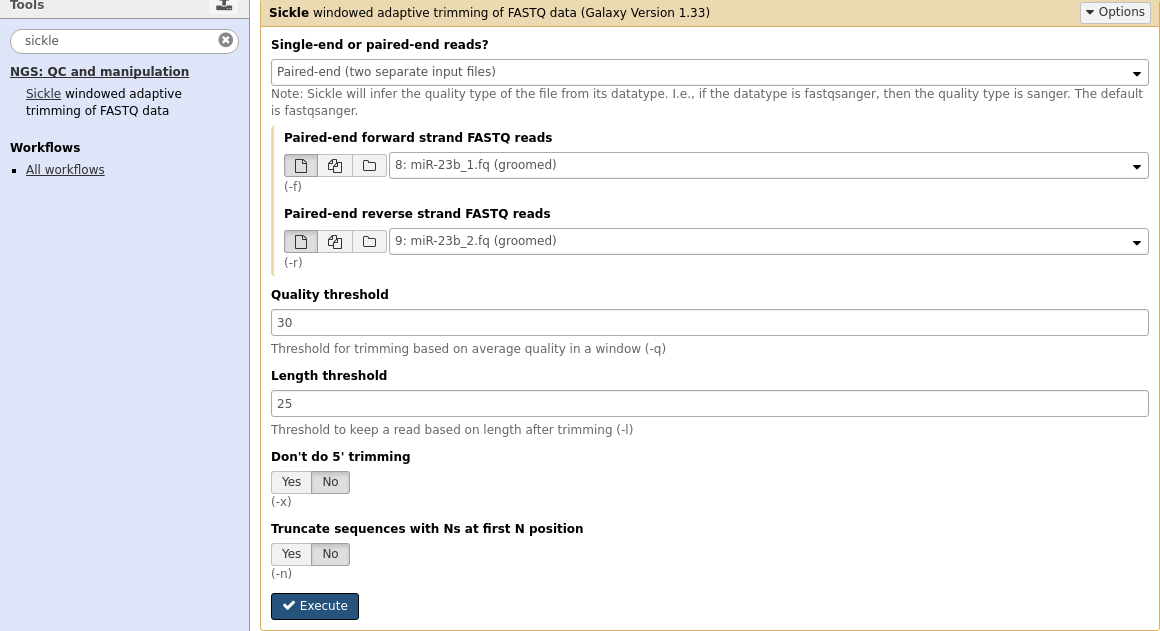
\includegraphics[width=\textwidth]{figures/qc_06.png}\\
After running a sickle analysis, rename the files 
\textit{Singletons from paired-end ...} and \textit{Paired-end output of Sickle on ...} to e.g.:
\begin{itemize}
	\item[] for miR-23b:
	\begin{itemize}
		\item miR-23b, singletons(clean)
		\item miR-23b\_1 (clean)
		\item miR-23b\_2 (clean)
	\end{itemize}
	\item[] for control sample:
	\begin{itemize}
		\item control sample, singletons(clean)
		\item control sample\_1 (clean)
		\item control sample\_2 (clean)
	\end{itemize}
\end{itemize}
If desired, you can hide the other results, such that you will get a history similar to:\\
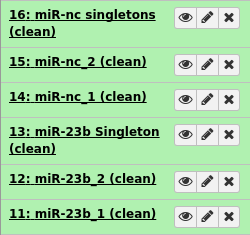
\includegraphics[scale=0.55]{figures/qc_07.png}\\
As you can see, Sickle produces for every set of paired sequencing reads, a set of pairs and an extra file with ``singletons''.
\begin{itemize}
	\item What would singletons be?
\end{itemize}
To confirm that the base quality has improved, run the FastQC again on \textit{ miR-23b (clean) }, and take a look at it:
\begin{itemize}
	\item Has the \textit{Per base sequence quality} improved?
	\item Have the per sequence quality scores improved?
	\item Why has the \textit{sequence length distribution} changed?
\end{itemize}
FastQC also has a section \textit{Overrepresented sequences}, indicated in red with a huge list. Apart from that we are using a truncated artificial dataset, it often happens in RNA-Seq data that these sequences appear. As said before, this tool was orignally written for DNA-Seq data.
\begin{itemize}
	\item Could you think of a reason why sequences could be overrepresented in RNA-Seq data?
\end{itemize}


% Module alignment:
\section{RNA-Seq: alignment}
To make more sense of the RNA-Seq data, we try to find the sequences back in the reference genome (mapping, aligning). The reference
genome should represent the most common sequence of the chromosomes of the human population. Please read the first paragraph (3 scentences) of the following url: \url{http://en.wikipedia.org/wiki/Reference_genome}
\begin{itemize}
	\item On how many individuals is hg19 based?
\end{itemize}
For RNA-Seq we need specialized RNA aligners, able to cope with gaps that originate from splicing. For this exercise we will make use of a tool called RNA-STAR. There are quite some of these aligners around. We will make use the tool ``\textit{\underline{HISAT2} A fast and sensitive alignment program}''. Load the aligner, select the following settings and leave the rest on default, and run an alignment for \textit{miR-23b (clean)} and \textit{control sample (clean)}. \textbf{Alignment is a computational very very heavy task so do NOT re-run or load it twice, or you have to give a treat:}\\
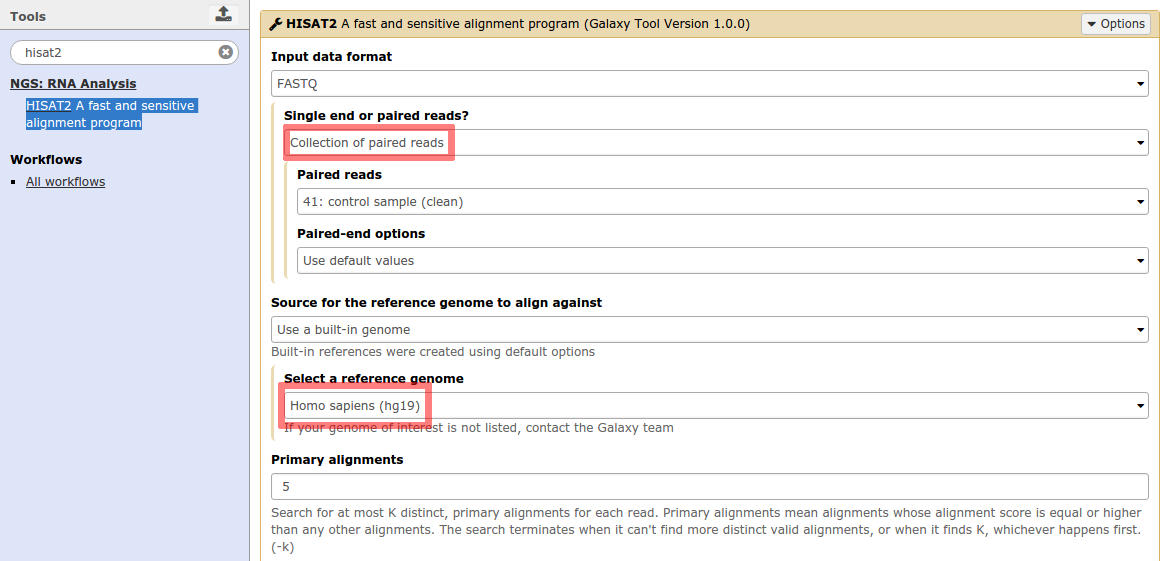
\includegraphics[width=\textwidth]{figures/alignment_01.png}\\
Please rename the \textit{HISAT2 on ...} to ``\textit{HISAT2 on miR-23b}'' and ``\textit{HISAT2 on control sample}''.
If the alignments do not have their \textbf{database} set, change it to hg19 as follows:\\
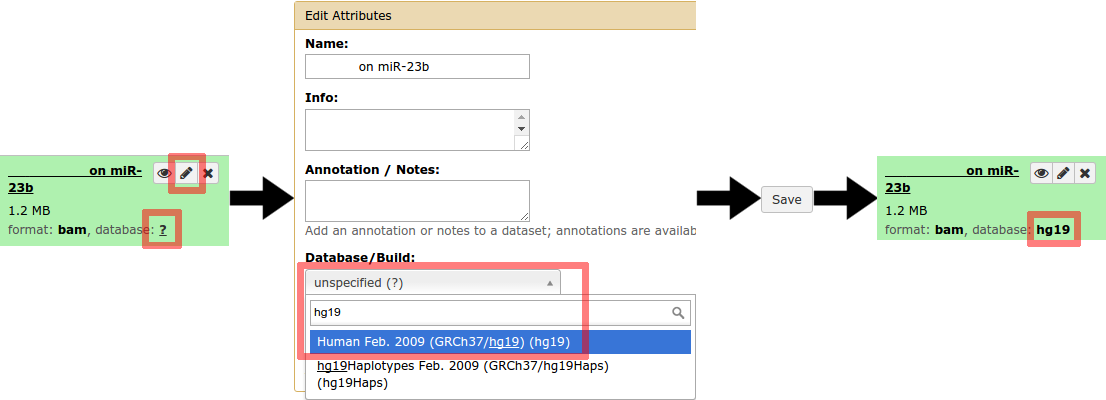
\includegraphics[width=\textwidth]{figures/alignment_02.png}\\
To get some general alignment statistics, run the tool ``\textit{\underline{Flagstat} tabulate descriptive stats for BAM datset}'' on \textit{HISAT2 on miR-23b}.
\begin{itemize}
	\item How many reads are multi-mapping?
\end{itemize}
For now we have only seen FastQ data and some summaries. To get an idea of what has been measured during the experiment, we can visualise the alignment. So, in the HISAT2 step we have been looking into hg19 where these sequences can be found in the reference genome, and this information is stored in those bam files. Start the built-in visualization Trackster at one of the alignments (make sure the dataset has \textbf{hg19} as database because we aligned to that):\\
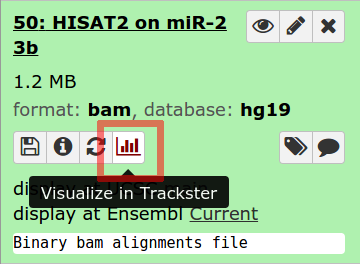
\includegraphics[scale=0.55]{figures/alignment_03}\\
Give it a name, press \textit{Create} and you show a yellow bar, indicating that the BAM file is being prepared. This means that the bam file is being convert into a file format that the browser can visualize. 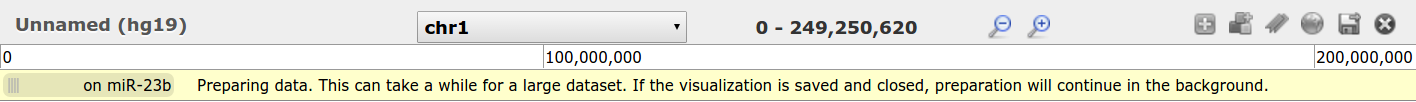
\includegraphics[width=\textwidth]{figures/alignment_04.png}\\
When this job is done, and it looks like this, make sure you save it:\\
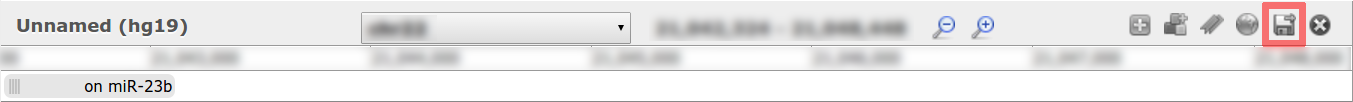
\includegraphics[width=\textwidth]{figures/alignment_05.png}\\
To add the other alignment, press the \textbf{[+]}-button:\\
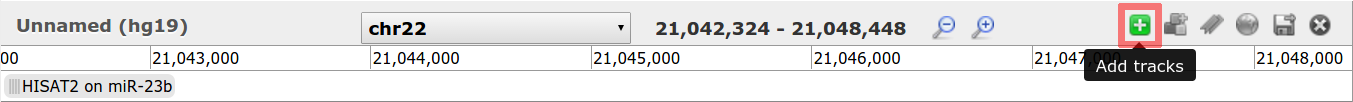
\includegraphics[width=\textwidth]{figures/alignment_06.png}\\
Now select the other alignment and press \textit{Add} and save it again:\\
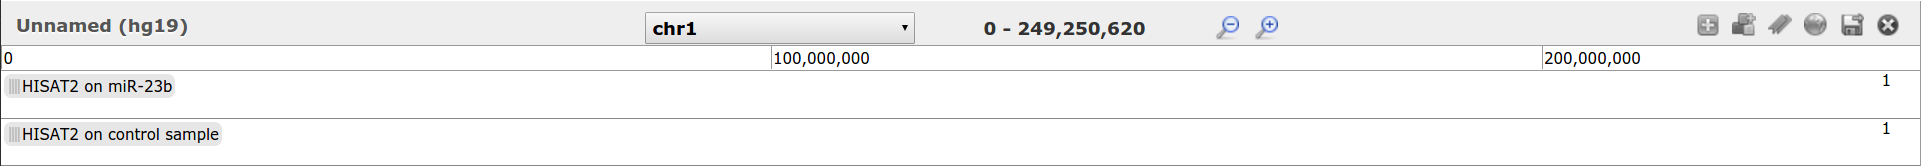
\includegraphics[width=\textwidth]{figures/alignment_07.png}\\
Remark that this is truncated data and you are supposed to see barely anything in here. Go to \textit{chr16}, to region \verb|chr16:15696870-15745667|.


% The singletons
%could be aligned separately in a single-end alignment, and could be added to the same alignment
%later on (but this is out of the scope of this tutorial). Go to Tophat2 and select Pair-end library. Make
%sure the reference genome is hg19. You have to run TWO alignments – one %for the quality trimmed
%“treat_” samples and one for the quality trimmed “ctrl_” samples.


%\bibliographystyle{natbib}
%\bibliographystyle{plainnat}

%\newpage

\vspace{-1.5em}
\bibliography{references}

\end{document}